\documentclass[JIP,draft]{ipsj}
\usepackage{graphicx}

\begin{document}
\title{Towards Cloud Bursting for Extreme Scale Supercomputers}

\begin{abstract}
Nowadays Supercomputers are widely used in scientifical computation, such as simulation and data analyse etc. 
Parallel programming are used to reduce execution time of complex problems, also fully utilizing computing resource of Supercomputers.
However, large serial applications will occupy computation nodes for a long time and causes some other applications which use numerous nodes to wait in a running queue, leads a low utilization of computing resource.
One solution is running virtual machine on 
In this paper, a comparision was made between a Public Cloud (AMAZON EC2) and a Supercomputer (TSUBAME) on Ethernet Performance and leading a 
\end{abstract}

\begin{keyword}
Supercomputer, Cloud, I/O Bursting Buffer Model
\end{keyword}

\maketitle

%1
\section{Introduction}
An increasing number of scientifical applications are now running on Supercomputer for high performance computing nodes, large bandwidth and low latency interconnection environment, also a great number of processors for high scalability.
High parallel application runs faster on Supercomputer for fully usage of computing resource.
However, it is usually difficult for a non-computer-scientist to write a parallel program, or re-write some existing applications into parallel version.
Many serial applications are submitted to Supercomputer and occupy computing nodes for a long time, casusing other applications which offer large number of nodes to wait for nodes, and leading a low utilization of computing resource.
One solution is running several virtual machines on a single physical machine for increasing utilization, which is used in TSUBAME Supercomputer.
However even using virtual machines computing nodes still can't meet the request of users, for example, power problem will be critial in summer and nearly half of computing nodes have be shutted down to reduce electricity consumation in the case of TSUBAME Supercomputer. 
Facing these problems, one solution will be federate supercomputer with public cloud.
By using pulic cloud computing nodes just in request peak or when facing with power problem, people can save cost for buying new machines.
Of cause, there will be many callenges when Supercomputer federates with public cloud, such as security problems, using public cloud may cause research data opened to public, also connecting with Internet put Supercomputer under threats of hacker's attack.


%2
\section{Background}

%3
\section{I/O Bursting Buffer Overview}
An overview of cloud environment and I/O Burst Buffer Model is described in this section.

\subsection{Cloud Environment}
First each cloud is defined as follow:


%For security consideration and the fact that IPv4 addresses becomes rare,
All computing nodes are connected by large bandwidth and interconnection network, note network topology maybe different in each cloud, so topology is not specifid here, interconnection network performance is measured by throughput.
There are a constant number of public IP addresses can be assigned to some computing nodes.
There is a shared storage for date sharing inside cloud, all computing nodes are connected with shared storage, also the filesystem of shared storage is not specified and performance is measured by throughput.


\subsection{I/O Bursting Buffer Archiecture}

\begin{figure}[tb]
	\centering
	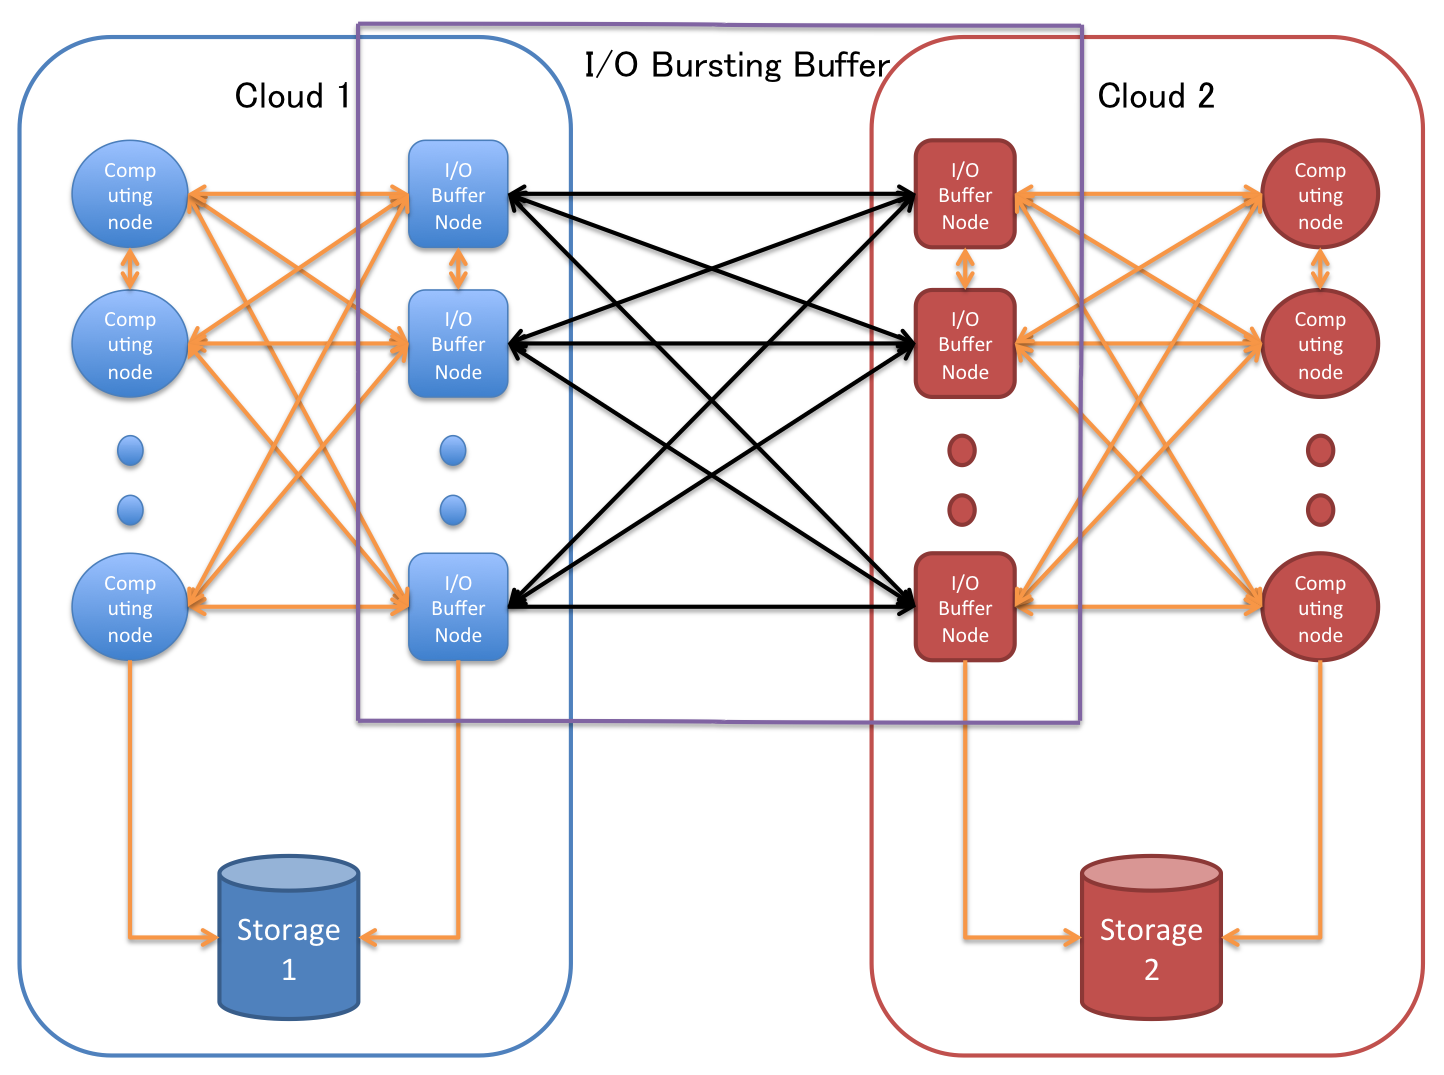
\includegraphics[width=6cm]{overview}
	\caption{overall illustrate of I/O Bursting Buffer Archiecture}
	\label{overview}
\end{figure}

Fig.~\ref{overview} is the overall illustrate of I/O Bursting Buffer Model

There are two clouds here, cloud condition is defined above.

Arrows stand for network connection.
Orange arrows are innerconnection networks inside cloud, although two clouds used the same color for innerconnection networks, bandwidth can be different, also the topolopies are not specified and can be different in each cloud.
Black arrows are Internet connections, since there are a few amount of public IP addresses avaliable, only I/O buffer nodes are connect to Internet, also the amount of avaliable public IP address becomes the upper bound of the amount of I/O buffer nodes in each cloud. 
Although nodes with private IP address can use route or other net device to connect to Internet, but consider about security problem, also using route will reduce concurrent data transfer rate, here we assume all nodes in cloud only connect to local private network except I/O buffer nodes which connect to both local network and Internet.

Circles stand for computing nodes, which are used for standard computation.
Here we assume all computing nodes can communicate with each other, and also I/O buffer nodes and shared storage in the same cloud environment.
Squares are I/O buffer nodes, these nodes are used for data transfer between clouds, and are assigned with both public and private IP addresses.
I/O buffer nodes can use the same machine or VM as computing nodes, or can use network optimized nodes for larger throughput, but it is not required here.
Cylinders are shared storages, which are used to store data used by computing nodes, .

For convenience, in the following section we assume data is stored in Cloud 1's shared storage, and computing nodes in Cloud 2 are used for computation. 

\section{I/O Bursting Buffer Model}

There are many facts will affect throughput of Internet, 

\subsection{data reading}

\begin{figure}[tb]
	\centering
	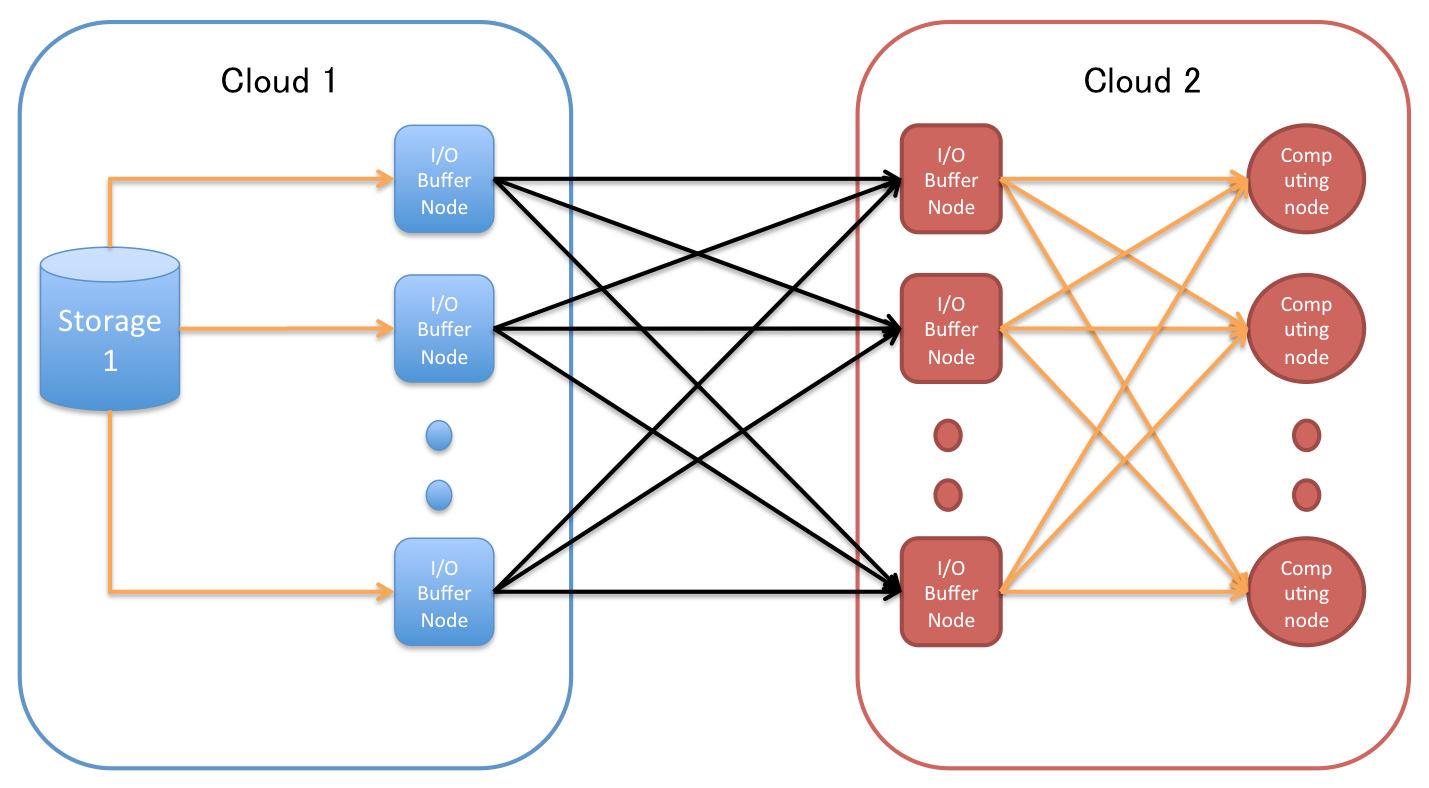
\includegraphics[width=8cm]{reading}
	\caption{data reading operation}
	\label{reading}
\end{figure}

When computing nodes issue read request, first we check whether the file has been cached in I/O buffer nodes in cloud 1, if not, File will be splited into the same number of I/O buffer nodes in cloud 1, and each I/O buffer node will be assgined a piece of split, then all I/O buffer nodes start reading assigned piece of data from shared storage simultaneously to fully utilize the bandwidth.

After transfering data from shared storage, a I/O buffer node in cloud 1 connects with all I/O buffer nodes in cloud 2, then split data piece and into number of I/O buffer nodes in cloud 2, and transfer these pieces to I/O buffer nodes in cloud 2 concurrently in order to fully utilize Internet bandwidth.


\end{document}
